% Topic 6.2: AI and Digital Finance
% Self-contained Beamer presentation
% Author: Joerg Osterrieder

\documentclass[11pt,aspectratio=169]{beamer}
\usetheme{Madrid}

% ======================= PACKAGES =======================
\usepackage{graphicx}
\usepackage{booktabs}
\usepackage{adjustbox}
\usepackage{multicol}
\usepackage{amsmath}
\usepackage{amssymb}
\usepackage{tikz}
\usetikzlibrary{arrows,shapes,positioning,shadows,trees}
\usepackage{listings}
\usepackage{xcolor}

% ======================= COLOR DEFINITIONS =======================
% Primary color scheme: Blue/Teal for Digital Finance
\definecolor{dfblue}{RGB}{0,102,204}
\definecolor{dfteal}{RGB}{0,153,153}
\definecolor{dfcyan}{RGB}{51,187,204}
\definecolor{dflightblue}{RGB}{153,204,255}
\definecolor{dflightblue2}{RGB}{173,214,255}
\definecolor{dflightblue3}{RGB}{193,224,255}
\definecolor{dflightblue4}{RGB}{213,234,255}

% Accent colors for finance applications
\definecolor{dfgreen}{RGB}{44, 160, 44}
\definecolor{dfred}{RGB}{214, 39, 40}
\definecolor{dforange}{RGB}{255, 127, 14}
\definecolor{dfgray}{RGB}{127, 127, 127}

% Utility colors
\definecolor{lightgray}{RGB}{240, 240, 240}
\definecolor{midgray}{RGB}{180, 180, 180}
\definecolor{codebg}{RGB}{245, 245, 245}

% ======================= THEME CUSTOMIZATION =======================
% Apply Digital Finance color scheme to Madrid theme
\setbeamercolor{palette primary}{bg=dflightblue3,fg=dfblue}
\setbeamercolor{palette secondary}{bg=dflightblue2,fg=dfblue}
\setbeamercolor{palette tertiary}{bg=dfteal,fg=white}
\setbeamercolor{palette quaternary}{bg=dfblue,fg=white}

\setbeamercolor{structure}{fg=dfblue}
\setbeamercolor{section in toc}{fg=dfblue}
\setbeamercolor{subsection in toc}{fg=dfteal}
\setbeamercolor{title}{fg=dfblue}
\setbeamercolor{frametitle}{fg=dfblue,bg=dflightblue3}
\setbeamercolor{block title}{bg=dflightblue2,fg=dfblue}
\setbeamercolor{block body}{bg=dflightblue4,fg=black}

% Remove navigation symbols for cleaner look
\setbeamertemplate{navigation symbols}{}

% Clean itemize/enumerate
\setbeamertemplate{itemize items}[circle]
\setbeamertemplate{enumerate items}[default]

% Margins for readability
\setbeamersize{text margin left=8mm,text margin right=8mm}

% ======================= LISTINGS CONFIGURATION =======================
% Python code style
\lstdefinestyle{pythonstyle}{
    language=Python,
    basicstyle=\ttfamily\footnotesize,
    keywordstyle=\color{dfblue}\bfseries,
    stringstyle=\color{dforange},
    commentstyle=\color{dfgray}\itshape,
    numberstyle=\tiny\color{dfgray},
    numbers=left,
    numbersep=5pt,
    backgroundcolor=\color{codebg},
    showspaces=false,
    showstringspaces=false,
    showtabs=false,
    frame=single,
    rulecolor=\color{midgray},
    tabsize=4,
    captionpos=b,
    breaklines=true,
    breakatwhitespace=false,
    escapeinside={(*@}{@*)},
    xleftmargin=10pt,
    xrightmargin=10pt
}

% Solidity code style
\lstdefinestyle{soliditystyle}{
    language=Java, % closest approximation
    basicstyle=\ttfamily\footnotesize,
    keywordstyle=\color{dfteal}\bfseries,
    stringstyle=\color{dforange},
    commentstyle=\color{dfgray}\itshape,
    numberstyle=\tiny\color{dfgray},
    numbers=left,
    numbersep=5pt,
    backgroundcolor=\color{codebg},
    showspaces=false,
    showstringspaces=false,
    showtabs=false,
    frame=single,
    rulecolor=\color{midgray},
    tabsize=2,
    captionpos=b,
    breaklines=true,
    breakatwhitespace=false,
    escapeinside={(*@}{@*)},
    xleftmargin=10pt,
    xrightmargin=10pt,
    morekeywords={pragma, contract, function, returns, public, private, view, pure, payable, address, uint256, mapping, event, modifier}
}

% Inline code command
\newcommand{\code}[1]{\texttt{\color{dfblue}#1}}

% ======================= CUSTOM COMMANDS =======================
% Bottom annotation (Madrid-style)
\newcommand{\bottomnote}[1]{%
\vfill
\vspace{-2mm}
\textcolor{dflightblue2}{\rule{\textwidth}{0.4pt}}
\vspace{1mm}
\footnotesize
\textbf{#1}
}

% Compact list spacing
\newcommand{\compactlist}{%
\setlength{\itemsep}{0pt}%
\setlength{\parskip}{0pt}%
\setlength{\parsep}{0pt}%
}

% Chart placeholder
\newcommand{\chartplaceholder}[2][5cm]{%
\begin{center}
\begin{adjustbox}{max width=0.95\textwidth, max height=#1}
\framebox[\textwidth][c]{%
\rule{0pt}{#1}%
\textcolor{midgray}{[#2]}%
}
\end{adjustbox}
\end{center}
}

% ======================= FINANCE NOTATION MACROS =======================
% Probability and statistics
\newcommand{\E}{\mathbb{E}} % Expected value
\newcommand{\Var}{\mathrm{Var}} % Variance
\newcommand{\Cov}{\mathrm{Cov}} % Covariance
\newcommand{\Prob}{\mathbb{P}} % Probability

% Distributions
\newcommand{\Normal}{\mathcal{N}} % Normal distribution
\newcommand{\Uniform}{\mathcal{U}} % Uniform distribution

% Returns and prices
\newcommand{\Ret}{R} % Return
\newcommand{\LogRet}{r} % Log return
\newcommand{\Price}{S} % Price/Stock price
\newcommand{\Strike}{K} % Strike price

% Options and derivatives
\newcommand{\CallPrice}{C} % Call option price
\newcommand{\PutPrice}{P} % Put option price
\newcommand{\Greeks}[1]{\mathit{#1}} % Greek letters

% Risk measures
\newcommand{\VaR}{\mathrm{VaR}} % Value at Risk
\newcommand{\CVaR}{\mathrm{CVaR}} % Conditional VaR
\newcommand{\Sharpe}{\mathrm{SR}} % Sharpe Ratio

% Time series
\newcommand{\AR}{\mathrm{AR}} % Autoregressive
\newcommand{\MA}{\mathrm{MA}} % Moving average
\newcommand{\GARCH}{\mathrm{GARCH}} % GARCH

% Blockchain/Crypto
\newcommand{\Hash}{\mathrm{Hash}} % Hash function
\newcommand{\Block}{\mathcal{B}} % Block
\newcommand{\Chain}{\mathcal{C}} % Chain

% Real numbers, integers
\newcommand{\R}{\mathbb{R}}
\newcommand{\Z}{\mathbb{Z}}
\newcommand{\N}{\mathbb{N}}

% ======================= TIKZ STYLES =======================
% Styles for finance-related diagrams
\tikzstyle{process} = [rectangle, minimum width=3cm, minimum height=1cm, text centered, draw=dfblue, fill=dflightblue4, thick]
\tikzstyle{decision} = [diamond, minimum width=3cm, minimum height=1cm, text centered, draw=dfteal, fill=dflightblue4, thick]
\tikzstyle{arrow} = [thick,->,>=stealth,color=dfblue]
\tikzstyle{blockchain} = [rectangle, rounded corners, minimum width=2.5cm, minimum height=1cm, text centered, draw=dfteal, fill=dflightblue3, thick]
\tikzstyle{transaction} = [circle, minimum size=0.8cm, text centered, draw=dforange, fill=dflightblue4, thick]

% ======================= FOOTER TEMPLATE =======================
\setbeamertemplate{footline}{
    \hbox{\begin{beamercolorbox}[wd=\paperwidth,ht=2.5ex,dp=1ex,leftskip=.5em,rightskip=.5em]{author in head/foot}
    \tiny
    \textbf{Digital Finance} \hfill
    Joerg Osterrieder \hfill
    \insertdate \hfill
    Page \insertframenumber{} / \inserttotalframenumber
    \end{beamercolorbox}}
}

% ======================= SECTION DIVIDER TEMPLATE =======================
\AtBeginSection[]{
\begin{frame}[plain]
\vfill
\centering
\begin{beamercolorbox}[sep=12pt,center]{title}
\usebeamerfont{title}\LARGE\insertsection\par
\end{beamercolorbox}
\vfill
\end{frame}
}


% ======================= ADDITIONAL STYLES =======================
\tikzstyle{aibox} = [rectangle, rounded corners, minimum width=2.5cm, minimum height=0.8cm, text centered, draw=dfpurple, fill=dfpurple!15, thick]
\definecolor{dfpurple}{RGB}{148, 103, 189}

% ======================= DOCUMENT INFO =======================
\title[Topic 6.2: AI in Finance]{Topic 6.2: AI and Digital Finance}
\subtitle{Machine Learning Transforms Financial Services}
\author{Joerg Osterrieder}
\institute{Digital Finance}
\date{2025}

\begin{document}

% =====================================================================
%                    SLIDE 1: TITLE SLIDE
% =====================================================================
\begin{frame}[plain]
\titlepage
\end{frame}

% =====================================================================
%                    SLIDE 2: LEARNING OBJECTIVES
% =====================================================================
\begin{frame}{Learning Objectives}
\begin{block}{By the end of this topic, you will be able to:}
\begin{enumerate}
\item \textbf{Identify} the major AI applications in finance (robo-advisory, fraud detection, credit scoring, algorithmic trading)
\item \textbf{Understand} the mathematical foundations of robo-advisors (Modern Portfolio Theory, mean-variance optimization)
\item \textbf{Analyze} AI risks including model opacity, adversarial attacks, and systemic risks
\item \textbf{Evaluate} AI claims in finance using a critical framework
\item \textbf{Apply} these concepts through hands-on robo-advisor simulation
\end{enumerate}
\end{block}

\vspace{0.3cm}
\textbf{Key Question:} How is artificial intelligence transforming financial services, and what are the associated risks and limitations?
\end{frame}

% =====================================================================
%                    SLIDE 3: PREREQUISITES
% =====================================================================
\begin{frame}{Prerequisites and Background}
\begin{columns}[T]
\begin{column}{0.48\textwidth}
\textbf{What You Should Know:}
\begin{itemize}
\item Basic understanding of financial markets
\item Concept of risk and return
\item Familiarity with portfolio diversification
\item Understanding of basic statistics (mean, variance, correlation)
\end{itemize}
\end{column}
\begin{column}{0.48\textwidth}
\textbf{Course Context:}
\begin{itemize}
\item Day 1: FinTech vs. DeFi landscape
\item Days 2-3: Blockchain and smart contracts
\item Day 4: Stablecoins and tokenization
\item Day 5: Regulation frameworks
\item \textbf{Today: AI as force multiplier}
\end{itemize}
\end{column}
\end{columns}

\vspace{0.5cm}
\begin{alertblock}{Connection to Previous Topics}
AI intersects with all previous material: AI-powered DeFi, algorithmic stablecoin management, automated compliance, and AI-driven trading on blockchain platforms.
\end{alertblock}
\end{frame}

% =====================================================================
%                    SLIDE 4: THE AI REVOLUTION IN FINANCE
% =====================================================================
\begin{frame}{The AI Revolution in Finance}
\begin{columns}[T]
\begin{column}{0.48\textwidth}
\textbf{Why AI Matters Now:}
\begin{itemize}
\item Massive data availability
\item Computational power explosion
\item Algorithm sophistication
\item Cost reduction pressure
\item Customer experience demands
\end{itemize}
\end{column}
\begin{column}{0.48\textwidth}
\textbf{Scale of Transformation:}
\begin{itemize}
\item \$1.4T+ in robo-advisor AUM (2024)
\item 75\%+ of trading volume algorithmic
\item Billions saved in fraud prevention
\item Millions gaining credit access
\end{itemize}
\end{column}
\end{columns}

\vspace{0.5cm}
\begin{block}{Critical Perspective}
AI in finance is both \textbf{genuinely transformative} and \textbf{frequently overhyped}. This topic gives you tools to distinguish between the two.
\end{block}
\end{frame}

% =====================================================================
%                    SLIDE 5: AI IN FINANCE LANDSCAPE
% =====================================================================
\begin{frame}{AI in Finance: The Landscape}
\begin{center}
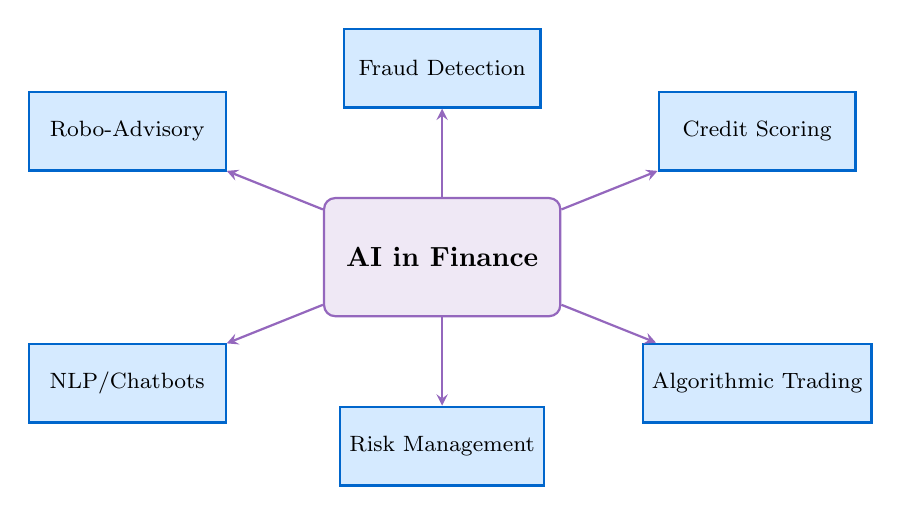
\begin{tikzpicture}[scale=0.8]
% Central AI node
\node[aibox, minimum width=3cm, minimum height=1.5cm, font=\bfseries] (ai) at (0,0) {AI in Finance};

% Applications around
\node[process, font=\footnotesize, minimum width=2.5cm] (robo) at (-5,2) {Robo-Advisory};
\node[process, font=\footnotesize, minimum width=2.5cm] (fraud) at (0,3) {Fraud Detection};
\node[process, font=\footnotesize, minimum width=2.5cm] (credit) at (5,2) {Credit Scoring};
\node[process, font=\footnotesize, minimum width=2.5cm] (trade) at (5,-2) {Algorithmic Trading};
\node[process, font=\footnotesize, minimum width=2.5cm] (risk) at (0,-3) {Risk Management};
\node[process, font=\footnotesize, minimum width=2.5cm] (nlp) at (-5,-2) {NLP/Chatbots};

% Connections
\draw[arrow, dfpurple] (ai) -- (robo);
\draw[arrow, dfpurple] (ai) -- (fraud);
\draw[arrow, dfpurple] (ai) -- (credit);
\draw[arrow, dfpurple] (ai) -- (trade);
\draw[arrow, dfpurple] (ai) -- (risk);
\draw[arrow, dfpurple] (ai) -- (nlp);
\end{tikzpicture}
\end{center}
\end{frame}

% =====================================================================
%                    SLIDE 6: ROBO-ADVISORY INTRODUCTION
% =====================================================================
\begin{frame}{AI Application 1: Robo-Advisory}
\begin{columns}[T]
\begin{column}{0.55\textwidth}
\begin{block}{What Is It?}
Automated investment management using algorithms to construct, monitor, and rebalance portfolios based on client goals and risk tolerance.
\end{block}

\textbf{How it works:}
\begin{enumerate}
\item Client inputs: goals, timeline, risk tolerance
\item Algorithm maps to asset allocation
\item Automated portfolio construction
\item Continuous monitoring and rebalancing
\item Tax-loss harvesting (if applicable)
\end{enumerate}
\end{column}
\begin{column}{0.42\textwidth}
\textbf{Key Players:}
\begin{itemize}
\item Betterment
\item Wealthfront
\item Schwab Intelligent Portfolios
\item Vanguard Digital Advisor
\end{itemize}

\vspace{0.3cm}
\textbf{Scale:}
\begin{itemize}
\item \$1.4T+ AUM globally (2024)
\item Fees: 0.25--0.50\% vs. 1\%+ traditional
\item Growing 20\%+ annually
\end{itemize}
\end{column}
\end{columns}

\bottomnote{See Notebook NB13 for hands-on robo-advisor simulation}
\end{frame}

% =====================================================================
%                    SLIDE 7: ROBO-ADVISORY MATH FOUNDATION
% =====================================================================
\begin{frame}{Robo-Advisory: The Math Behind It}
\textbf{Mean-Variance Optimization (Markowitz):}
\begin{equation}
\min_w \frac{1}{2} w^T \Sigma w - \lambda \mu^T w
\end{equation}
\begin{itemize}
\item $w$ = portfolio weights
\item $\Sigma$ = covariance matrix of returns
\item $\mu$ = expected returns vector
\item $\lambda$ = risk aversion parameter
\end{itemize}

\vspace{0.3cm}
\textbf{Mapping Risk Tolerance to $\lambda$:}
\begin{table}[h]
\centering
\small
\begin{tabular}{lcc}
\toprule
\textbf{Risk Profile} & \textbf{$\lambda$} & \textbf{Typical Equity \%} \\
\midrule
Conservative & 1--2 & 20--40\% \\
Moderate & 3--5 & 40--60\% \\
Aggressive & 6--10 & 60--90\% \\
\bottomrule
\end{tabular}
\end{table}

\bottomnote{Modern robo-advisors add constraints: factor exposure, ESG filters, tax efficiency}
\end{frame}

% =====================================================================
%                    SLIDE 8: PORTFOLIO RETURN AND VARIANCE
% =====================================================================
\begin{frame}{Portfolio Mathematics: Return and Variance}
\begin{columns}[T]
\begin{column}{0.48\textwidth}
\textbf{Portfolio Expected Return:}
\begin{equation}
r_p = w^T \mu = \sum_{i=1}^{n} w_i \mu_i
\end{equation}

\vspace{0.3cm}
\textbf{Portfolio Variance:}
\begin{equation}
\sigma_p^2 = w^T \Sigma w
\end{equation}

\vspace{0.3cm}
\textbf{Key Insight:}\\
Diversification reduces $\sigma_p^2$ through off-diagonal covariance terms when correlations are less than 1.
\end{column}
\begin{column}{0.48\textwidth}
\textbf{The Sharpe Ratio:}
\begin{equation}
\text{SR} = \frac{r_p - r_f}{\sigma_p}
\end{equation}
\begin{itemize}
\item $r_p$ = portfolio return
\item $r_f$ = risk-free rate (e.g., T-bills)
\item $\sigma_p$ = portfolio volatility
\end{itemize}

\vspace{0.3cm}
\textbf{Interpretation:}\\
Excess return per unit of risk. Higher is better.
\end{column}
\end{columns}
\end{frame}

% =====================================================================
%                    SLIDE 9: EFFICIENT FRONTIER
% =====================================================================
\begin{frame}{The Efficient Frontier}
\begin{columns}[T]
\begin{column}{0.55\textwidth}
\begin{center}
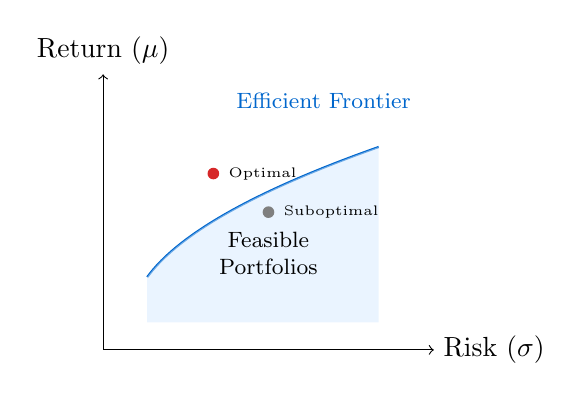
\begin{tikzpicture}[scale=0.7]
% Axes
\draw[->] (0,0) -- (6,0) node[right] {Risk ($\sigma$)};
\draw[->] (0,0) -- (0,5) node[above] {Return ($\mu$)};

% Efficient frontier curve
\draw[thick, dfblue, domain=0.8:5, samples=50] plot (\x, {0.5 + 1.5*sqrt(\x - 0.5)});

% Inefficient region
\fill[dflightblue4, opacity=0.5] (0.8,0.5) -- plot[domain=0.8:5, samples=50] (\x, {0.5 + 1.5*sqrt(\x - 0.5)}) -- (5,0.5) -- cycle;

% Labels
\node[above, font=\footnotesize, dfblue] at (4,4.2) {Efficient Frontier};
\node[font=\footnotesize] at (3,2) {Feasible};
\node[font=\footnotesize] at (3,1.5) {Portfolios};

% Points
\fill[dfred] (2,3.2) circle (3pt);
\node[right, font=\tiny] at (2.1,3.2) {Optimal};
\fill[dfgray] (3,2.5) circle (3pt);
\node[right, font=\tiny] at (3.1,2.5) {Suboptimal};
\end{tikzpicture}
\end{center}
\end{column}
\begin{column}{0.42\textwidth}
\textbf{Definition:}\\
The set of portfolios that maximize return for a given risk level, or minimize risk for a given return.

\vspace{0.3cm}
\textbf{Key Properties:}
\begin{itemize}
\item Portfolios below are suboptimal
\item Portfolios above are impossible
\item Rational investors choose only frontier portfolios
\end{itemize}
\end{column}
\end{columns}
\end{frame}

% =====================================================================
%                    SLIDE 10: RISK PROFILING
% =====================================================================
\begin{frame}{Risk Profiling: From Questionnaire to Portfolio}
\begin{columns}[T]
\begin{column}{0.48\textwidth}
\textbf{Risk Assessment Factors:}
\begin{enumerate}
\item Investment time horizon
\item Reaction to hypothetical losses
\item Financial goals (growth vs. income)
\item Investment experience
\item Income stability
\item Liquidity needs
\end{enumerate}
\end{column}
\begin{column}{0.48\textwidth}
\textbf{Scoring Methodology:}
\begin{table}[h]
\centering
\footnotesize
\begin{tabular}{lc}
\toprule
\textbf{Score Range} & \textbf{Profile} \\
\midrule
0--20 & Conservative \\
21--40 & Moderately Conservative \\
41--60 & Moderate \\
61--80 & Moderately Aggressive \\
81--100 & Aggressive \\
\bottomrule
\end{tabular}
\end{table}
\end{column}
\end{columns}

\vspace{0.3cm}
\begin{block}{From Score to Portfolio}
Each risk profile maps to a target asset allocation (e.g., 60/40 stocks/bonds), which then drives the mean-variance optimization with appropriate constraints.
\end{block}
\end{frame}

% =====================================================================
%                    SLIDE 11: REBALANCING STRATEGIES
% =====================================================================
\begin{frame}{Portfolio Rebalancing Strategies}
\begin{columns}[T]
\begin{column}{0.48\textwidth}
\textbf{Calendar-Based:}
\begin{itemize}
\item Rebalance on fixed schedule
\item Monthly, quarterly, or annually
\item Simple to implement
\item May miss significant drifts
\end{itemize}

\vspace{0.3cm}
\textbf{Threshold-Based:}
\begin{itemize}
\item Rebalance when drift exceeds threshold
\item Typically 5\% deviation trigger
\item More responsive to market moves
\item Minimizes unnecessary trading
\end{itemize}
\end{column}
\begin{column}{0.48\textwidth}
\textbf{Hybrid Approach:}
\begin{itemize}
\item Check thresholds daily
\item Mandatory annual review
\item Tax-efficient timing
\item Cash flow integration
\end{itemize}

\vspace{0.3cm}
\begin{alertblock}{Trade-off}
More frequent rebalancing = better risk control but higher costs. Robo-advisors optimize this balance automatically.
\end{alertblock}
\end{column}
\end{columns}
\end{frame}

% =====================================================================
%                    SLIDE 12: TAX-LOSS HARVESTING
% =====================================================================
\begin{frame}{Tax-Loss Harvesting}
\begin{block}{Definition}
Selling investments at a loss to offset capital gains and reduce taxes, then replacing with similar assets to maintain market exposure.
\end{block}

\begin{columns}[T]
\begin{column}{0.48\textwidth}
\textbf{How It Works:}
\begin{enumerate}
\item Identify positions with unrealized losses
\item Sell to realize the loss
\item Immediately buy similar (not identical) asset
\item Use loss to offset gains
\end{enumerate}
\end{column}
\begin{column}{0.48\textwidth}
\textbf{The Wash Sale Rule:}
\begin{itemize}
\item Cannot buy ``substantially identical'' security within 30 days before/after sale
\item Loss disallowed if violated
\item Solution: Use similar but not identical ETFs
\end{itemize}
\end{column}
\end{columns}

\vspace{0.3cm}
\textbf{Robo-Advisor Advantage:} Automated systems can monitor all positions daily and harvest losses systematically---impractical for human advisors at scale.
\end{frame}

% =====================================================================
%                    SLIDE 13: ROBO-ADVISOR FEE COMPARISON
% =====================================================================
\begin{frame}{Fee Comparison: Robo vs. Traditional}
\begin{columns}[T]
\begin{column}{0.55\textwidth}
\begin{table}[h]
\centering
\small
\begin{tabular}{lcc}
\toprule
\textbf{Service Type} & \textbf{Annual Fee} \\
\midrule
Pure Robo-Advisor & 0.15--0.50\% \\
Hybrid Robo + Human & 0.30--0.50\% \\
Independent RIA & 0.50--1.50\% \\
Traditional Broker & 1.00--2.00\% \\
Private Wealth Mgmt & 1.00--2.50\% \\
\bottomrule
\end{tabular}
\end{table}
\end{column}
\begin{column}{0.42\textwidth}
\textbf{Long-Term Impact:}\\
On \$100,000 over 30 years at 7\% return:

\vspace{0.2cm}
\begin{itemize}
\item 0.25\% fee: \$700,000 final
\item 1.00\% fee: \$574,000 final
\item \textbf{Difference: \$126,000}
\end{itemize}

\vspace{0.3cm}
\textbf{The Compounding Effect:}\\
Small fee differences compound into large wealth differences over time.
\end{column}
\end{columns}
\end{frame}

% =====================================================================
%                    SLIDE 14: FRAUD DETECTION
% =====================================================================
\begin{frame}{AI Application 2: Fraud Detection}
\begin{columns}[T]
\begin{column}{0.48\textwidth}
\textbf{Traditional Rules-Based:}
\begin{itemize}
\item If transaction > \$10,000 $\rightarrow$ flag
\item If international + new merchant $\rightarrow$ flag
\item Static thresholds
\item High false positive rate
\item Easily gamed once known
\end{itemize}
\end{column}
\begin{column}{0.48\textwidth}
\textbf{ML-Based Detection:}
\begin{itemize}
\item Learns from historical fraud patterns
\item Dynamic thresholds per user
\item Behavioral biometrics
\item Network analysis
\item Adapts to new attack vectors
\end{itemize}
\end{column}
\end{columns}

\vspace{0.5cm}
\begin{block}{Common ML Approaches}
\begin{itemize}
\item \textbf{Supervised}: Random forests, gradient boosting, neural networks on labeled fraud data
\item \textbf{Unsupervised}: Anomaly detection (isolation forests, autoencoders)
\item \textbf{Graph-based}: Network analysis to detect fraud rings
\end{itemize}
\end{block}
\end{frame}

% =====================================================================
%                    SLIDE 15: FRAUD DETECTION METRICS
% =====================================================================
\begin{frame}{Fraud Detection: Performance Metrics}
\begin{columns}[T]
\begin{column}{0.48\textwidth}
\textbf{Key Metrics:}
\begin{itemize}
\item \textbf{Precision}: Of flagged transactions, how many are actually fraud?
\item \textbf{Recall}: Of all fraud, how much do we catch?
\item \textbf{False Positive Rate}: Legitimate transactions incorrectly flagged
\end{itemize}

\vspace{0.3cm}
\textbf{The Trade-off:}\\
Higher recall (catching more fraud) typically increases false positives (blocking legitimate users).
\end{column}
\begin{column}{0.48\textwidth}
\textbf{Industry Benchmarks:}
\begin{table}[h]
\centering
\footnotesize
\begin{tabular}{lcc}
\toprule
\textbf{System} & \textbf{Recall} & \textbf{FPR} \\
\midrule
Rules-based & 60\% & 5\% \\
Basic ML & 85\% & 2\% \\
Advanced ML & 95\% & 0.5\% \\
\bottomrule
\end{tabular}
\end{table}

\vspace{0.2cm}
\textbf{Business Impact:}\\
Reducing FPR from 5\% to 0.5\% = 90\% fewer frustrated customers.
\end{column}
\end{columns}
\end{frame}

% =====================================================================
%                    SLIDE 16: CREDIT SCORING
% =====================================================================
\begin{frame}{AI Application 3: Credit Scoring}
\begin{columns}[T]
\begin{column}{0.48\textwidth}
\textbf{Traditional FICO:}
\begin{itemize}
\item Payment history (35\%)
\item Amounts owed (30\%)
\item Length of history (15\%)
\item New credit (10\%)
\item Credit mix (10\%)
\end{itemize}

\vspace{0.2cm}
\textbf{Limitations:}
\begin{itemize}
\item ``Credit invisible'' populations
\item Backward-looking only
\item Limited data sources
\end{itemize}
\end{column}
\begin{column}{0.48\textwidth}
\textbf{AI/Alternative Data Scoring:}
\begin{itemize}
\item Bank transaction patterns
\item Utility/rent payment history
\item Employment data
\item Education records
\item Behavioral signals
\item Social connections
\end{itemize}

\vspace{0.2cm}
\textbf{Players:}
\begin{itemize}
\item Upstart, ZestFinance, Lenddo
\item Claims: 75\% fewer defaults at same approval rate
\end{itemize}
\end{column}
\end{columns}
\end{frame}

% =====================================================================
%                    SLIDE 17: CREDIT SCORING ETHICAL CONCERNS
% =====================================================================
\begin{frame}{Credit Scoring: Ethical and Legal Considerations}
\begin{columns}[T]
\begin{column}{0.48\textwidth}
\textbf{Potential Benefits:}
\begin{itemize}
\item Financial inclusion for ``thin file'' consumers
\item More accurate risk assessment
\item Lower costs passed to consumers
\item Faster decisions
\end{itemize}
\end{column}
\begin{column}{0.48\textwidth}
\textbf{Potential Risks:}
\begin{itemize}
\item Proxy discrimination
\item Lack of transparency
\item Data privacy concerns
\item Perpetuating historical biases
\end{itemize}
\end{column}
\end{columns}

\vspace{0.3cm}
\begin{alertblock}{Regulatory Requirements}
\begin{itemize}
\item \textbf{ECOA} (US): Cannot discriminate on race, religion, national origin, sex
\item \textbf{FCRA} (US): Right to know reasons for adverse actions
\item \textbf{GDPR} (EU): Right to explanation for automated decisions
\end{itemize}
\end{alertblock}
\end{frame}

% =====================================================================
%                    SLIDE 18: ALGORITHMIC TRADING
% =====================================================================
\begin{frame}{AI Application 4: Algorithmic Trading}
\begin{columns}[T]
\begin{column}{0.55\textwidth}
\textbf{Evolution of Quant Trading:}
\begin{enumerate}
\item \textbf{1980s--90s}: Statistical arbitrage
\item \textbf{2000s}: High-frequency trading
\item \textbf{2010s}: Factor investing at scale
\item \textbf{2020s}: Deep learning, NLP, alternative data
\end{enumerate}

\vspace{0.3cm}
\textbf{Modern AI Trading Signals:}
\begin{itemize}
\item Satellite imagery (parking lots, shipping)
\item Social media sentiment
\item Patent filings, job postings
\item Earnings call NLP analysis
\item Web traffic data
\end{itemize}
\end{column}
\begin{column}{0.42\textwidth}
\begin{alertblock}{Reality Check}
\begin{itemize}
\item Most AI trading strategies don't beat benchmarks net of fees
\item Overfitting is rampant
\item Alpha decays quickly once discovered
\item Data quality issues pervasive
\end{itemize}
\end{alertblock}

\textbf{Institutional players:}\\
Two Sigma, Citadel, Renaissance, DE Shaw
\end{column}
\end{columns}
\end{frame}

% =====================================================================
%                    SLIDE 19: ALGORITHMIC TRADING STRATEGIES
% =====================================================================
\begin{frame}{Algorithmic Trading: Strategy Types}
\begin{columns}[T]
\begin{column}{0.32\textwidth}
\textbf{Market Making:}
\begin{itemize}
\item Provide liquidity
\item Earn bid-ask spread
\item High frequency
\item Low margin, high volume
\end{itemize}
\end{column}
\begin{column}{0.32\textwidth}
\textbf{Statistical Arbitrage:}
\begin{itemize}
\item Exploit price relationships
\item Mean reversion
\item Pairs trading
\item Market neutral
\end{itemize}
\end{column}
\begin{column}{0.32\textwidth}
\textbf{Momentum/Trend:}
\begin{itemize}
\item Follow price trends
\item Technical signals
\item Factor-based
\item Longer holding periods
\end{itemize}
\end{column}
\end{columns}

\vspace{0.5cm}
\begin{block}{The Alpha Challenge}
\begin{itemize}
\item Markets are highly efficient
\item Any profitable pattern gets arbitraged away
\item Need continuous innovation to maintain edge
\item Most retail AI trading systems fail
\end{itemize}
\end{block}
\end{frame}

% =====================================================================
%                    SLIDE 20: AI IN DEFI
% =====================================================================
\begin{frame}{AI in DeFi: Emerging Applications}
\begin{columns}[T]
\begin{column}{0.48\textwidth}
\textbf{Current Applications:}
\begin{itemize}
\item MEV (Maximal Extractable Value) bots
\item Liquidation bots
\item Yield farming optimizers
\item Portfolio rebalancing agents
\item Smart contract auditing
\end{itemize}
\end{column}
\begin{column}{0.48\textwidth}
\textbf{Emerging/Experimental:}
\begin{itemize}
\item AI-managed DAOs
\item Autonomous trading agents
\item On-chain ML inference
\item LLM-powered governance
\item AI agents holding wallets
\end{itemize}
\end{column}
\end{columns}

\vspace{0.5cm}
\begin{exampleblock}{Example: Yearn Finance}
Yearn uses algorithms to automatically move deposits between yield strategies, optimizing for the highest risk-adjusted returns. Not ``AI'' in the deep learning sense, but algorithmic automation of DeFi.
\end{exampleblock}
\end{frame}

% =====================================================================
%                    SLIDE 21: MODEL OPACITY RISK
% =====================================================================
\begin{frame}{AI Risks in Finance: Model Opacity}
\begin{block}{The Black Box Problem}
Complex ML models (neural networks, gradient boosting) often cannot explain \emph{why} they make specific predictions. This creates regulatory and ethical challenges.
\end{block}

\begin{columns}[T]
\begin{column}{0.48\textwidth}
\textbf{Why It Matters:}
\begin{itemize}
\item Regulatory requirements (ECOA, GDPR)
\item Right to explanation for credit denials
\item Model risk management
\item Debugging and improvement
\item Trust and accountability
\end{itemize}
\end{column}
\begin{column}{0.48\textwidth}
\textbf{Mitigation Approaches:}
\begin{itemize}
\item Interpretable models (logistic regression)
\item SHAP/LIME explanations
\item Surrogate models
\item Feature importance analysis
\item Regulatory sandboxes
\end{itemize}
\end{column}
\end{columns}

\vspace{0.3cm}
\centering
\textbf{Tension:} More complex models $\rightarrow$ better predictions $\rightarrow$ less interpretability
\end{frame}

% =====================================================================
%                    SLIDE 22: ADVERSARIAL ATTACKS
% =====================================================================
\begin{frame}{AI Risks in Finance: Adversarial Attacks}
\begin{block}{Definition}
Deliberately crafted inputs designed to fool ML models while appearing normal to humans.
\end{block}

\begin{columns}[T]
\begin{column}{0.48\textwidth}
\textbf{Finance-Specific Threats:}
\begin{itemize}
\item \textbf{Credit fraud}: Manipulate application to get approval
\item \textbf{Trading}: Poison training data with fake signals
\item \textbf{KYC bypass}: Adversarial images for identity verification
\item \textbf{Spam}: Evade NLP-based filters
\end{itemize}
\end{column}
\begin{column}{0.48\textwidth}
\textbf{Example: Credit Application}
\begin{itemize}
\item Attacker knows model features
\item Slightly modifies spending patterns
\item Opens strategic accounts
\item Model sees ``good'' applicant
\item Fraud not detected until default
\end{itemize}
\end{column}
\end{columns}

\vspace{0.3cm}
\begin{alertblock}{Deepfake Fraud}
AI-generated voice/video for social engineering attacks. A CFO ``calls'' to authorize a wire transfer---but it's a deepfake. Losses in the tens of millions already documented.
\end{alertblock}
\end{frame}

% =====================================================================
%                    SLIDE 23: SYSTEMIC RISKS
% =====================================================================
\begin{frame}{AI Risks: Systemic and Concentration}
\begin{columns}[T]
\begin{column}{0.48\textwidth}
\textbf{Herding Risk:}
\begin{itemize}
\item Many firms use similar models
\item Trained on same data
\item Similar predictions $\rightarrow$ same trades
\item Amplifies market moves
\item Flash crashes
\end{itemize}

\vspace{0.3cm}
\textbf{Historical Example:}\\
August 2007 quant meltdown---many funds used similar factor models, simultaneous deleveraging.
\end{column}
\begin{column}{0.48\textwidth}
\textbf{Concentration Risk:}
\begin{itemize}
\item Few dominant AI providers
\item Cloud infrastructure concentration
\item Model monoculture
\item Single points of failure
\end{itemize}

\vspace{0.3cm}
\textbf{Regulatory Response:}
\begin{itemize}
\item EU AI Act (risk classification)
\item Fed/OCC model risk guidance
\item Explainability requirements
\end{itemize}
\end{column}
\end{columns}
\end{frame}

% =====================================================================
%                    SLIDE 24: CRITICAL EVALUATION FRAMEWORK
% =====================================================================
\begin{frame}{AI Claims: A Critical Evaluation Framework}
\textbf{When you hear ``AI will disrupt X in finance,'' ask:}

\begin{enumerate}
\item \textbf{What's the benchmark?} Is AI actually better than existing methods, or just newer?
\item \textbf{Is there enough data?} ML needs large, clean datasets. Rare events (like financial crises) are hard to learn from.
\item \textbf{Is the environment stationary?} Financial markets change; models trained on past data may fail.
\item \textbf{What are the feedback loops?} If everyone uses the same AI, does it still work?
\item \textbf{What's the adversarial dynamic?} Are there incentives to game the model?
\item \textbf{What's the regulatory status?} Can this legally be deployed?
\end{enumerate}

\vspace{0.3cm}
\begin{alertblock}{Healthy Skepticism}
Most AI finance claims are overhyped. Demand evidence: backtests (with proper methodology), out-of-sample performance, real-world deployments.
\end{alertblock}
\end{frame}

% =====================================================================
%                    SLIDE 25: HANDS-ON EXERCISE INTRO
% =====================================================================
\begin{frame}{Hands-On: Robo-Advisor Simulation (NB13)}
\textbf{What you'll do in the notebook:}
\begin{enumerate}
\item Load historical return data for major asset classes
\item Implement mean-variance optimization
\item Map risk tolerance scores to portfolio allocations
\item Visualize efficient frontier
\item Simulate portfolio performance under different risk profiles
\item Add constraints (position limits, ESG filters)
\end{enumerate}

\vspace{0.3cm}
\begin{block}{Key Learning Objectives}
\begin{itemize}
\item Understand how robo-advisors translate preferences to portfolios
\item See the math behind automated investing
\item Recognize the assumptions and limitations
\end{itemize}
\end{block}

\bottomnote{Notebook: NB13\_Robo\_Advisor\_Simulation.ipynb}
\end{frame}

% =====================================================================
%                    SLIDE 26: HANDS-ON EXERCISE DETAILS
% =====================================================================
\begin{frame}{NB13: Implementation Details}
\begin{columns}[T]
\begin{column}{0.48\textwidth}
\textbf{Data Used:}
\begin{itemize}
\item US Stocks (SPY proxy)
\item International Stocks (VEU)
\item US Bonds (AGG)
\item International Bonds (BWX)
\item Real Estate (VNQ)
\item Commodities (GSG)
\end{itemize}

\vspace{0.2cm}
\textbf{Time Period:}\\
10+ years of daily returns for robust estimation
\end{column}
\begin{column}{0.48\textwidth}
\textbf{Key Code Steps:}
\begin{enumerate}
\item Calculate $\mu$ (expected returns)
\item Estimate $\Sigma$ (covariance matrix)
\item Solve optimization problem
\item Generate efficient frontier
\item Map risk scores to allocations
\item Backtest performance
\end{enumerate}

\vspace{0.2cm}
\textbf{Extensions:}
\begin{itemize}
\item Add position limits
\item Implement rebalancing
\item Add tax-loss harvesting
\end{itemize}
\end{column}
\end{columns}
\end{frame}

% =====================================================================
%                    SLIDE 27: DISCUSSION - AI VS HUMAN
% =====================================================================
\begin{frame}{Discussion: AI vs. Human Advisors}
\begin{columns}[T]
\begin{column}{0.48\textwidth}
\begin{block}{Robo-Advisor Advantages}
\begin{itemize}
\item Lower costs (0.25\% vs. 1\%+)
\item No minimum investment barriers
\item Consistent, disciplined execution
\item 24/7 availability
\item No emotional decision-making
\item Tax optimization at scale
\end{itemize}
\end{block}
\end{column}
\begin{column}{0.48\textwidth}
\begin{block}{Human Advisor Advantages}
\begin{itemize}
\item Complex financial planning
\item Behavioral coaching
\item Life event guidance
\item Estate and tax planning
\item Relationship and trust
\item Flexibility for unique situations
\end{itemize}
\end{block}
\end{column}
\end{columns}

\vspace{0.3cm}
\begin{exampleblock}{The Hybrid Model}
Leading platforms now offer ``hybrid'' services combining algorithmic management with human advice access (e.g., Vanguard Personal Advisor Services at 0.30\%).
\end{exampleblock}
\end{frame}

% =====================================================================
%                    SLIDE 28: DISCUSSION - MARKET IMPLICATIONS
% =====================================================================
\begin{frame}{Discussion: Market-Wide Implications of AI}
\begin{columns}[T]
\begin{column}{0.48\textwidth}
\textbf{Efficiency Arguments:}
\begin{itemize}
\item Better price discovery
\item Increased liquidity
\item Lower transaction costs
\item Faster information incorporation
\item Reduced human error
\end{itemize}
\end{column}
\begin{column}{0.48\textwidth}
\textbf{Stability Concerns:}
\begin{itemize}
\item Flash crashes
\item Correlated strategies
\item Feedback loops
\item Reduced diversity of views
\item Unknown failure modes
\end{itemize}
\end{column}
\end{columns}

\vspace{0.5cm}
\begin{block}{Discussion Questions}
\begin{enumerate}
\item Does AI make markets more or less stable?
\item Should there be ``speed limits'' on algorithmic trading?
\item Who is liable when AI systems cause market disruptions?
\end{enumerate}
\end{block}
\end{frame}

% =====================================================================
%                    SLIDE 29: APPLICATION - CAREER IMPLICATIONS
% =====================================================================
\begin{frame}{Application: Career Implications}
\begin{columns}[T]
\begin{column}{0.48\textwidth}
\textbf{Jobs at Risk of Automation:}
\begin{itemize}
\item Basic financial analysis
\item Routine trading operations
\item Standard compliance checking
\item Simple customer service
\item Manual data entry
\end{itemize}
\end{column}
\begin{column}{0.48\textwidth}
\textbf{Growing Demand:}
\begin{itemize}
\item AI/ML engineers in finance
\item Quantitative developers
\item Model risk managers
\item AI ethics specialists
\item Human-AI interface designers
\end{itemize}
\end{column}
\end{columns}

\vspace{0.5cm}
\begin{block}{Key Skills for the Future}
\begin{itemize}
\item Combination of finance domain knowledge + technical skills
\item Understanding of AI capabilities AND limitations
\item Ability to explain complex models to stakeholders
\item Critical thinking about AI claims
\end{itemize}
\end{block}
\end{frame}

% =====================================================================
%                    SLIDE 30: APPLICATION - REGULATORY LANDSCAPE
% =====================================================================
\begin{frame}{Application: Regulatory Landscape for AI in Finance}
\begin{columns}[T]
\begin{column}{0.48\textwidth}
\textbf{Current Frameworks:}
\begin{itemize}
\item \textbf{US}: SEC guidance on robo-advisors; Fed SR 11-7 on model risk
\item \textbf{EU}: MiFID II suitability; GDPR data rights; EU AI Act
\item \textbf{UK}: FCA guidance on AI/ML
\item \textbf{Global}: FSB reports on AI/ML risks
\end{itemize}
\end{column}
\begin{column}{0.48\textwidth}
\textbf{Key Requirements:}
\begin{itemize}
\item Suitability assessments
\item Disclosure of algorithmic use
\item Explainability for adverse actions
\item Model risk management
\item Fair lending compliance
\item Data protection
\end{itemize}
\end{column}
\end{columns}

\vspace{0.3cm}
\begin{alertblock}{EU AI Act Classification}
Financial AI applications (credit scoring, insurance pricing) are classified as ``high-risk'' requiring conformity assessments, transparency, and human oversight.
\end{alertblock}
\end{frame}

% =====================================================================
%                    SLIDE 31: EXECUTIVE SUMMARY
% =====================================================================
\begin{frame}{Executive Summary}
\begin{block}{Key Takeaways from Topic 6.2}
\begin{enumerate}
\item \textbf{AI applications} span robo-advisory, fraud detection, credit scoring, and algorithmic trading---each with distinct benefits and risks
\item \textbf{Robo-advisors} democratize investment management through Modern Portfolio Theory, reducing fees from 1\%+ to 0.25\%
\item \textbf{ML in credit scoring} can expand access but raises fairness and explainability concerns
\item \textbf{Algorithmic trading} dominates markets but most strategies fail to beat benchmarks
\item \textbf{Key risks} include model opacity, adversarial attacks, systemic herding, and concentration
\item \textbf{Critical evaluation} is essential---most AI claims are overhyped
\end{enumerate}
\end{block}

\vspace{0.3cm}
\centering
\textbf{Bottom Line:} AI is transforming finance, but with clear limitations and risks that require careful management.
\end{frame}

% =====================================================================
%                    SLIDE 32: CONCEPT MAP
% =====================================================================
\begin{frame}{Concept Map: AI and Digital Finance}
\begin{center}
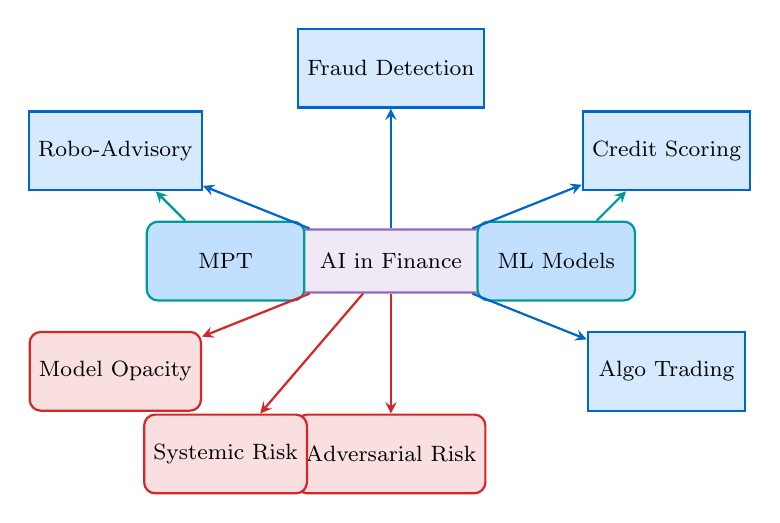
\begin{tikzpicture}[scale=0.7, every node/.style={font=\footnotesize}]
% Central node
\node[aibox, minimum width=2.5cm] (center) at (0,0) {AI in Finance};

% Applications
\node[process, minimum width=2cm] (robo) at (-5,2) {Robo-Advisory};
\node[process, minimum width=2cm] (fraud) at (0,3.5) {Fraud Detection};
\node[process, minimum width=2cm] (credit) at (5,2) {Credit Scoring};
\node[process, minimum width=2cm] (algo) at (5,-2) {Algo Trading};

% Risks
\node[blockchain, minimum width=2cm, draw=dfred, fill=dfred!15] (opacity) at (-5,-2) {Model Opacity};
\node[blockchain, minimum width=2cm, draw=dfred, fill=dfred!15] (adv) at (0,-3.5) {Adversarial Risk};
\node[blockchain, minimum width=2cm, draw=dfred, fill=dfred!15] (sys) at (-3,-3.5) {Systemic Risk};

% Foundations
\node[blockchain, minimum width=2cm] (mpt) at (-3,0) {MPT};
\node[blockchain, minimum width=2cm] (ml) at (3,0) {ML Models};

% Connections
\draw[arrow] (center) -- (robo);
\draw[arrow] (center) -- (fraud);
\draw[arrow] (center) -- (credit);
\draw[arrow] (center) -- (algo);
\draw[arrow, dfred] (center) -- (opacity);
\draw[arrow, dfred] (center) -- (adv);
\draw[arrow, dfred] (center) -- (sys);
\draw[arrow, dfteal] (mpt) -- (robo);
\draw[arrow, dfteal] (ml) -- (credit);
\end{tikzpicture}
\end{center}
\end{frame}

% =====================================================================
%                    SLIDE 33: KEY TERMS (1)
% =====================================================================
\begin{frame}{Key Terms (1/2)}
\begin{description}
\item[Robo-Advisor] Automated platform providing digital investment management using algorithms to construct and rebalance portfolios

\item[Modern Portfolio Theory (MPT)] Framework for constructing portfolios to maximize return for a given risk level through diversification

\item[Mean-Variance Optimization] Mathematical approach to find optimal portfolio weights by balancing expected return against variance

\item[Efficient Frontier] Set of optimal portfolios offering highest return for each level of risk

\item[Sharpe Ratio] Risk-adjusted return measure: $(r_p - r_f) / \sigma_p$

\item[Tax-Loss Harvesting] Selling losing investments to realize losses for tax benefits while maintaining market exposure
\end{description}
\end{frame}

% =====================================================================
%                    SLIDE 34: KEY TERMS (2)
% =====================================================================
\begin{frame}{Key Terms (2/2)}
\begin{description}
\item[Wash Sale Rule] IRS rule prohibiting repurchase of substantially identical securities within 30 days of selling at a loss

\item[Alternative Data] Non-traditional data sources (satellite imagery, social media, web traffic) used for financial predictions

\item[Model Opacity] Inability to explain why complex ML models make specific predictions (``black box'' problem)

\item[Adversarial Attack] Deliberately crafted inputs designed to fool ML models

\item[Herding Risk] Systemic risk from many institutions using similar AI models and making correlated decisions

\item[SHAP/LIME] Techniques for explaining individual predictions from complex ML models
\end{description}
\end{frame}

% =====================================================================
%                    SLIDE 35: COMMON MISCONCEPTIONS
% =====================================================================
\begin{frame}{Common Misconceptions}
\begin{columns}[T]
\begin{column}{0.48\textwidth}
\begin{alertblock}{Misconception 1}
``AI trading systems consistently beat the market''
\end{alertblock}
\textbf{Reality:} Most fail after accounting for transaction costs, fees, and survivorship bias. Markets are highly efficient.

\vspace{0.3cm}
\begin{alertblock}{Misconception 2}
``More data always means better predictions''
\end{alertblock}
\textbf{Reality:} Data quality matters more than quantity. Noisy, biased, or non-stationary data can harm models.
\end{column}
\begin{column}{0.48\textwidth}
\begin{alertblock}{Misconception 3}
``AI removes human bias from finance''
\end{alertblock}
\textbf{Reality:} AI can amplify historical biases present in training data, potentially creating systematic discrimination.

\vspace{0.3cm}
\begin{alertblock}{Misconception 4}
``Robo-advisors are only for small investors''
\end{alertblock}
\textbf{Reality:} Sophisticated investors increasingly use algorithmic tools; the technology scales to any portfolio size.
\end{column}
\end{columns}
\end{frame}

% =====================================================================
%                    SLIDE 36: SELF-ASSESSMENT (1)
% =====================================================================
\begin{frame}{Self-Assessment Questions (1/2)}
\begin{block}{Question 1 (From Quiz 6.2, Q2)}
What is the typical annual fee range for robo-advisors compared to traditional advisors?
\begin{enumerate}[A.]
\item Robo: 2-3\%, Traditional: 4-5\%
\item Robo: 0.15-0.50\%, Traditional: 1.00-2.00\%
\item Robo: 5-10\%, Traditional: 1-2\%
\item Both charge the same: 1-2\%
\end{enumerate}
\end{block}

\vspace{0.3cm}
\begin{block}{Question 2 (From Quiz 6.2, Q8)}
In the Sharpe ratio formula $(r_p - r_f) / \sigma_p$, what does $r_f$ typically represent?
\begin{enumerate}[A.]
\item The inflation rate
\item The expected market return
\item The risk-free rate, such as the Treasury bill rate
\item The firm's cost of capital
\end{enumerate}
\end{block}
\end{frame}

% =====================================================================
%                    SLIDE 37: SELF-ASSESSMENT (2)
% =====================================================================
\begin{frame}{Self-Assessment Questions (2/2)}
\begin{block}{Question 3 (From Quiz 6.2, Q17)}
What is the Black-Litterman model used for in advanced robo-advisors?
\begin{enumerate}[A.]
\item Predicting stock prices with 100\% accuracy
\item Combining market equilibrium returns with investor views to create more stable portfolio allocations
\item Calculating transaction costs
\item Determining tax rates for different investments
\end{enumerate}
\end{block}

\vspace{0.5cm}
\begin{exampleblock}{Answers}
\begin{itemize}
\item Question 1: \textbf{B} -- Robo-advisors charge 0.15-0.50\%, significantly less than traditional 1-2\%
\item Question 2: \textbf{C} -- The risk-free rate (typically T-bills) is the baseline return with no risk
\item Question 3: \textbf{B} -- Black-Litterman combines equilibrium returns with investor views for stability
\end{itemize}
\end{exampleblock}
\end{frame}

% =====================================================================
%                    SLIDE 38: WHAT'S NEXT
% =====================================================================
\begin{frame}{What's Next: Topic 6.3 -- Synthesis Framework}
\begin{columns}[T]
\begin{column}{0.48\textwidth}
\textbf{Preview of T6.3:}
\begin{itemize}
\item Building your digital finance worldview
\item The Innovation Scorecard framework
\item Six questions for any innovation
\item Applying multiple analytical lenses
\item Capstone exercise (NB14)
\end{itemize}
\end{column}
\begin{column}{0.48\textwidth}
\textbf{Connection to Today:}
\begin{itemize}
\item AI as one technology to evaluate
\item Framework applies to AI claims
\item Integration with regulatory lens
\item Critical evaluation skills
\end{itemize}
\end{column}
\end{columns}

\vspace{0.5cm}
\begin{block}{Preparation}
Think about how you would evaluate a new AI-powered financial service:
\begin{itemize}
\item What problem does it solve?
\item What are the risks and tradeoffs?
\item Who benefits and who bears costs?
\end{itemize}
\end{block}
\end{frame}

% =====================================================================
%                    SLIDE 39: RESOURCES
% =====================================================================
\begin{frame}{Resources for Further Learning}
\begin{columns}[T]
\begin{column}{0.48\textwidth}
\textbf{Academic/Technical:}
\begin{itemize}
\item Markowitz, H. (1952) ``Portfolio Selection''
\item Black \& Litterman (1992) ``Global Portfolio Optimization''
\item Advances in Financial Machine Learning (Lopez de Prado)
\item Journal of Financial Economics
\end{itemize}

\vspace{0.3cm}
\textbf{Industry Reports:}
\begin{itemize}
\item FSB: ``Artificial Intelligence and Machine Learning in Financial Services''
\item BIS: ``Big Tech in Finance''
\item Federal Reserve: SR 11-7 (Model Risk Management)
\end{itemize}
\end{column}
\begin{column}{0.48\textwidth}
\textbf{Practical/News:}
\begin{itemize}
\item Risk.net (AI in finance coverage)
\item The Block, CoinDesk (AI+crypto)
\item a16z crypto blog
\item MIT Technology Review
\end{itemize}

\vspace{0.3cm}
\textbf{Tools and Platforms:}
\begin{itemize}
\item Python: PyPortfolioOpt, cvxpy
\item Betterment, Wealthfront (try them)
\item Quantopian archives
\item QuantConnect (algo trading)
\end{itemize}
\end{column}
\end{columns}
\end{frame}

% =====================================================================
%                    SLIDE 40: QUESTIONS
% =====================================================================
\begin{frame}{}
\vfill
\begin{center}
{\Huge Questions?}

\vspace{1cm}

{\large Topic 6.2: AI and Digital Finance}

\vspace{0.5cm}

{\normalsize Machine Learning Transforms Financial Services}

\vspace{1cm}

\textbf{Next:} Topic 6.3 -- Building Your Digital Finance Worldview

\vspace{0.5cm}

\textcolor{dfgray}{Joerg Osterrieder | Digital Finance | 2025}
\end{center}
\vfill
\end{frame}

\end{document}
